\documentclass[1p]{elsarticle_modified}
%\bibliographystyle{elsarticle-num}

%\usepackage[colorlinks]{hyperref}
%\usepackage{abbrmath_seonhwa} %\Abb, \Ascr, \Acal ,\Abf, \Afrak
\usepackage{amsfonts}
\usepackage{amssymb}
\usepackage{amsmath}
\usepackage{amsthm}
\usepackage{scalefnt}
\usepackage{amsbsy}
\usepackage{kotex}
\usepackage{caption}
\usepackage{subfig}
\usepackage{color}
\usepackage{graphicx}
\usepackage{xcolor} %% white, black, red, green, blue, cyan, magenta, yellow
\usepackage{float}
\usepackage{setspace}
\usepackage{hyperref}

\usepackage{tikz}
\usetikzlibrary{arrows}

\usepackage{multirow}
\usepackage{array} % fixed length table
\usepackage{hhline}

%%%%%%%%%%%%%%%%%%%%%
\makeatletter
\renewcommand*\env@matrix[1][\arraystretch]{%
	\edef\arraystretch{#1}%
	\hskip -\arraycolsep
	\let\@ifnextchar\new@ifnextchar
	\array{*\c@MaxMatrixCols c}}
\makeatother %https://tex.stackexchange.com/questions/14071/how-can-i-increase-the-line-spacing-in-a-matrix
%%%%%%%%%%%%%%%

\usepackage[normalem]{ulem}

\newcommand{\msout}[1]{\ifmmode\text{\sout{\ensuremath{#1}}}\else\sout{#1}\fi}
%SOURCE: \msout is \stkout macro in https://tex.stackexchange.com/questions/20609/strikeout-in-math-mode

\newcommand{\cancel}[1]{
	\ifmmode
	{\color{red}\msout{#1}}
	\else
	{\color{red}\sout{#1}}
	\fi
}

\newcommand{\add}[1]{
	{\color{blue}\uwave{#1}}
}

\newcommand{\replace}[2]{
	\ifmmode
	{\color{red}\msout{#1}}{\color{blue}\uwave{#2}}
	\else
	{\color{red}\sout{#1}}{\color{blue}\uwave{#2}}
	\fi
}

\newcommand{\Sol}{\mathcal{S}} %segment
\newcommand{\D}{D} %diagram
\newcommand{\A}{\mathcal{A}} %arc


%%%%%%%%%%%%%%%%%%%%%%%%%%%%%5 test

\def\sl{\operatorname{\textup{SL}}(2,\Cbb)}
\def\psl{\operatorname{\textup{PSL}}(2,\Cbb)}
\def\quan{\mkern 1mu \triangleright \mkern 1mu}

\theoremstyle{definition}
\newtheorem{thm}{Theorem}[section]
\newtheorem{prop}[thm]{Proposition}
\newtheorem{lem}[thm]{Lemma}
\newtheorem{ques}[thm]{Question}
\newtheorem{cor}[thm]{Corollary}
\newtheorem{defn}[thm]{Definition}
\newtheorem{exam}[thm]{Example}
\newtheorem{rmk}[thm]{Remark}
\newtheorem{alg}[thm]{Algorithm}

\newcommand{\I}{\sqrt{-1}}
\begin{document}

%\begin{frontmatter}
%
%\title{Boundary parabolic representations of knots up to 8 crossings}
%
%%% Group authors per affiliation:
%\author{Yunhi Cho} 
%\address{Department of Mathematics, University of Seoul, Seoul, Korea}
%\ead{yhcho@uos.ac.kr}
%
%
%\author{Seonhwa Kim} %\fnref{s_kim}}
%\address{Center for Geometry and Physics, Institute for Basic Science, Pohang, 37673, Korea}
%\ead{ryeona17@ibs.re.kr}
%
%\author{Hyuk Kim}
%\address{Department of Mathematical Sciences, Seoul National University, Seoul 08826, Korea}
%\ead{hyukkim@snu.ac.kr}
%
%\author{Seokbeom Yoon}
%\address{Department of Mathematical Sciences, Seoul National University, Seoul, 08826,  Korea}
%\ead{sbyoon15@snu.ac.kr}
%
%\begin{abstract}
%We find all boundary parabolic representation of knots up to 8 crossings.
%
%\end{abstract}
%\begin{keyword}
%    \MSC[2010] 57M25 
%\end{keyword}
%
%\end{frontmatter}

%\linenumbers
%\tableofcontents
%
\newcommand\colored[1]{\textcolor{white}{\rule[-0.35ex]{0.8em}{1.4ex}}\kern-0.8em\color{red} #1}%
%\newcommand\colored[1]{\textcolor{white}{ #1}\kern-2.17ex	\textcolor{white}{ #1}\kern-1.81ex	\textcolor{white}{ #1}\kern-2.15ex\color{red}#1	}

{\Large $\underline{12a_{0523}~(K12a_{0523})}$}

\setlength{\tabcolsep}{10pt}
\renewcommand{\arraystretch}{1.6}
\vspace{1cm}\begin{tabular}{m{100pt}>{\centering\arraybackslash}m{274pt}}
\multirow{5}{120pt}{
	\centering
	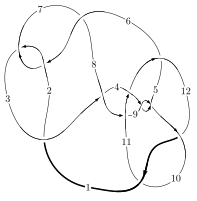
\includegraphics[width=112pt]{../../../GIT/diagram.site/Diagrams/png/1324_12a_0523.png}\\
\ \ \ A knot diagram\footnotemark}&
\allowdisplaybreaks
\textbf{Linearized knot diagam} \\
\cline{2-2}
 &
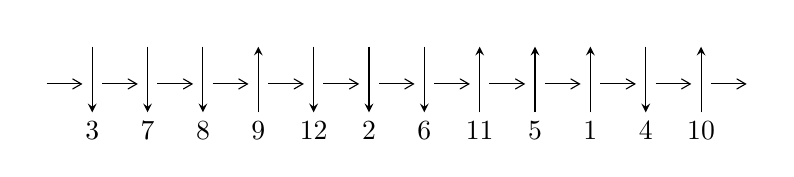
\begin{tikzpicture}[x=20pt, y=17pt]
	% nodes
	\node (C0) at (0, 0) {};
	\node (C1) at (1, 0) {};
	\node (C1U) at (1, +1) {};
	\node (C1D) at (1, -1) {3};

	\node (C2) at (2, 0) {};
	\node (C2U) at (2, +1) {};
	\node (C2D) at (2, -1) {7};

	\node (C3) at (3, 0) {};
	\node (C3U) at (3, +1) {};
	\node (C3D) at (3, -1) {8};

	\node (C4) at (4, 0) {};
	\node (C4U) at (4, +1) {};
	\node (C4D) at (4, -1) {9};

	\node (C5) at (5, 0) {};
	\node (C5U) at (5, +1) {};
	\node (C5D) at (5, -1) {12};

	\node (C6) at (6, 0) {};
	\node (C6U) at (6, +1) {};
	\node (C6D) at (6, -1) {2};

	\node (C7) at (7, 0) {};
	\node (C7U) at (7, +1) {};
	\node (C7D) at (7, -1) {6};

	\node (C8) at (8, 0) {};
	\node (C8U) at (8, +1) {};
	\node (C8D) at (8, -1) {11};

	\node (C9) at (9, 0) {};
	\node (C9U) at (9, +1) {};
	\node (C9D) at (9, -1) {5};

	\node (C10) at (10, 0) {};
	\node (C10U) at (10, +1) {};
	\node (C10D) at (10, -1) {1};

	\node (C11) at (11, 0) {};
	\node (C11U) at (11, +1) {};
	\node (C11D) at (11, -1) {4};

	\node (C12) at (12, 0) {};
	\node (C12U) at (12, +1) {};
	\node (C12D) at (12, -1) {10};
	\node (C13) at (13, 0) {};

	% arrows
	\draw[->,>={angle 60}]
	(C0) edge (C1) (C1) edge (C2) (C2) edge (C3) (C3) edge (C4) (C4) edge (C5) (C5) edge (C6) (C6) edge (C7) (C7) edge (C8) (C8) edge (C9) (C9) edge (C10) (C10) edge (C11) (C11) edge (C12) (C12) edge (C13) ;	\draw[->,>=stealth]
	(C1U) edge (C1D) (C2U) edge (C2D) (C3U) edge (C3D) (C4D) edge (C4U) (C5U) edge (C5D) (C6U) edge (C6D) (C7U) edge (C7D) (C8D) edge (C8U) (C9D) edge (C9U) (C10D) edge (C10U) (C11U) edge (C11D) (C12D) edge (C12U) ;
	\end{tikzpicture} \\
\hhline{~~} \\& 
\textbf{Solving Sequence} \\ \cline{2-2} 
 &
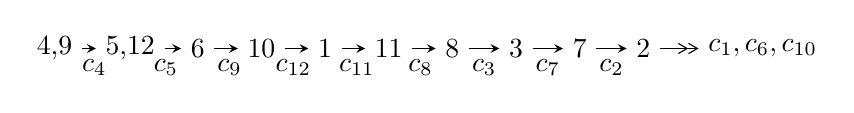
\begin{tikzpicture}[x=23pt, y=7pt]
	% node
	\node (A0) at (-1/8, 0) {4,9};
	\node (A1) at (17/16, 0) {5,12};
	\node (A2) at (17/8, 0) {6};
	\node (A3) at (25/8, 0) {10};
	\node (A4) at (33/8, 0) {1};
	\node (A5) at (41/8, 0) {11};
	\node (A6) at (49/8, 0) {8};
	\node (A7) at (57/8, 0) {3};
	\node (A8) at (65/8, 0) {7};
	\node (A9) at (73/8, 0) {2};
	\node (C1) at (1/2, -1) {$c_{4}$};
	\node (C2) at (13/8, -1) {$c_{5}$};
	\node (C3) at (21/8, -1) {$c_{9}$};
	\node (C4) at (29/8, -1) {$c_{12}$};
	\node (C5) at (37/8, -1) {$c_{11}$};
	\node (C6) at (45/8, -1) {$c_{8}$};
	\node (C7) at (53/8, -1) {$c_{3}$};
	\node (C8) at (61/8, -1) {$c_{7}$};
	\node (C9) at (69/8, -1) {$c_{2}$};
	\node (A10) at (11, 0) {$c_{1},c_{6},c_{10}$};

	% edge
	\draw[->,>=stealth]	
	(A0) edge (A1) (A1) edge (A2) (A2) edge (A3) (A3) edge (A4) (A4) edge (A5) (A5) edge (A6) (A6) edge (A7) (A7) edge (A8) (A8) edge (A9) ;
	\draw[->>,>={angle 60}]	
	(A9) edge (A10);
\end{tikzpicture} \\ 

\end{tabular} \\

\footnotetext{
The image of knot diagram is generated by the software ``\textbf{Draw programme}" developed by Andrew Bartholomew(\url{http://www.layer8.co.uk/maths/draw/index.htm\#Running-draw}), where we modified some parts for our purpose(\url{https://github.com/CATsTAILs/LinksPainter}).
}\phantom \\ \newline 
\centering \textbf{Ideals for irreducible components\footnotemark of $X_{\text{par}}$} 
 
\begin{align*}
I^u_{1}&=\langle 
-6.53596\times10^{293} u^{104}+7.87917\times10^{293} u^{103}+\cdots+2.51893\times10^{295} b+4.10389\times10^{293},\\
\phantom{I^u_{1}}&\phantom{= \langle  }5.19190\times10^{296} u^{104}-1.30156\times10^{297} u^{103}+\cdots+7.80867\times10^{296} a+2.98862\times10^{296},\\
\phantom{I^u_{1}}&\phantom{= \langle  }u^{105}-2 u^{104}+\cdots+3 u^2+1\rangle \\
I^u_{2}&=\langle 
b,\;a+1,\;u+1\rangle \\
\\
\end{align*}
\raggedright * 2 irreducible components of $\dim_{\mathbb{C}}=0$, with total 106 representations.\\
\footnotetext{All coefficients of polynomials are rational numbers. But the coefficients are sometimes approximated in decimal forms when there is not enough margin.}
\newpage
\renewcommand{\arraystretch}{1}
\centering \section*{I. $I^u_{1}= \langle -6.54\times10^{293} u^{104}+7.88\times10^{293} u^{103}+\cdots+2.52\times10^{295} b+4.10\times10^{293},\;5.19\times10^{296} u^{104}-1.30\times10^{297} u^{103}+\cdots+7.81\times10^{296} a+2.99\times10^{296},\;u^{105}-2 u^{104}+\cdots+3 u^2+1 \rangle$}
\flushleft \textbf{(i) Arc colorings}\\
\begin{tabular}{m{7pt} m{180pt} m{7pt} m{180pt} }
\flushright $a_{4}=$&$\begin{pmatrix}1\\0\end{pmatrix}$ \\
\flushright $a_{9}=$&$\begin{pmatrix}0\\u\end{pmatrix}$ \\
\flushright $a_{5}=$&$\begin{pmatrix}1\\- u^2\end{pmatrix}$ \\
\flushright $a_{12}=$&$\begin{pmatrix}-0.664889 u^{104}+1.66681 u^{103}+\cdots+1.49798 u-0.382731\\0.0259474 u^{104}-0.0312799 u^{103}+\cdots+2.02082 u-0.0162922\end{pmatrix}$ \\
\flushright $a_{6}=$&$\begin{pmatrix}-4.30965 u^{104}+4.08364 u^{103}+\cdots+3.79930 u+8.10925\\0.0507263 u^{104}-0.0723374 u^{103}+\cdots-0.0688675 u-0.0910713\end{pmatrix}$ \\
\flushright $a_{10}=$&$\begin{pmatrix}u\\- u^3+u\end{pmatrix}$ \\
\flushright $a_{1}=$&$\begin{pmatrix}-0.675206 u^{104}+1.69171 u^{103}+\cdots+0.487482 u-0.370705\\- u^3+u\end{pmatrix}$ \\
\flushright $a_{11}=$&$\begin{pmatrix}-0.638941 u^{104}+1.63553 u^{103}+\cdots+3.51880 u-0.399023\\0.0259474 u^{104}-0.0312799 u^{103}+\cdots+2.02082 u-0.0162922\end{pmatrix}$ \\
\flushright $a_{8}=$&$\begin{pmatrix}5.02213 u^{104}-5.76629 u^{103}+\cdots-14.5025 u-3.74387\\-0.0685443 u^{104}+0.0806585 u^{103}+\cdots-0.927508 u+0.0754778\end{pmatrix}$ \\
\flushright $a_{3}=$&$\begin{pmatrix}1.84791 u^{104}-1.44973 u^{103}+\cdots-1.12604 u-1.51565\\-0.104549 u^{104}+0.0699046 u^{103}+\cdots+0.0417599 u+0.0704983\end{pmatrix}$ \\
\flushright $a_{7}=$&$\begin{pmatrix}5.89546 u^{104}-6.94305 u^{103}+\cdots-11.8346 u-4.93404\\-0.278081 u^{104}+0.312953 u^{103}+\cdots-0.771699 u+0.279228\end{pmatrix}$ \\
\flushright $a_{2}=$&$\begin{pmatrix}1.53539 u^{104}-0.555872 u^{103}+\cdots-2.03889 u-2.74853\\-0.0668628 u^{104}+0.0559341 u^{103}+\cdots+0.951702 u+0.0225999\end{pmatrix}$\\&\end{tabular}
\flushleft \textbf{(ii) Obstruction class $= -1$}\\~\\
\flushleft \textbf{(iii) Cusp Shapes $= 3.59047 u^{104}-1.27532 u^{103}+\cdots+8.64459 u-8.12545$}\\~\\
\newpage\renewcommand{\arraystretch}{1}
\flushleft \textbf{(iv) u-Polynomials at the component}\newline \\
\begin{tabular}{m{50pt}|m{274pt}}
Crossings & \hspace{64pt}u-Polynomials at each crossing \\
\hline $$\begin{aligned}c_{1},c_{7}\end{aligned}$$&$\begin{aligned}
&u^{105}+34 u^{104}+\cdots-6 u+1
\end{aligned}$\\
\hline $$\begin{aligned}c_{2},c_{6}\end{aligned}$$&$\begin{aligned}
&u^{105}-2 u^{104}+\cdots+2 u-1
\end{aligned}$\\
\hline $$\begin{aligned}c_{3}\end{aligned}$$&$\begin{aligned}
&u^{105}+4 u^{104}+\cdots-317390 u-19141
\end{aligned}$\\
\hline $$\begin{aligned}c_{4},c_{9}\end{aligned}$$&$\begin{aligned}
&u^{105}-2 u^{104}+\cdots+3 u^2+1
\end{aligned}$\\
\hline $$\begin{aligned}c_{5}\end{aligned}$$&$\begin{aligned}
&31(31 u^{105}+196 u^{104}+\cdots+3.96866\times10^{7} u+4806371)
\end{aligned}$\\
\hline $$\begin{aligned}c_{8}\end{aligned}$$&$\begin{aligned}
&31(31 u^{105}-196 u^{104}+\cdots-554872 u-22063)
\end{aligned}$\\
\hline $$\begin{aligned}c_{10},c_{12}\end{aligned}$$&$\begin{aligned}
&u^{105}+3 u^{104}+\cdots+1098 u-81
\end{aligned}$\\
\hline $$\begin{aligned}c_{11}\end{aligned}$$&$\begin{aligned}
&u^{105}+3 u^{104}+\cdots+1440 u+279
\end{aligned}$\\
\hline
\end{tabular}\\~\\
\newpage\renewcommand{\arraystretch}{1}
\flushleft \textbf{(v) Riley Polynomials at the component}\newline \\
\begin{tabular}{m{50pt}|m{274pt}}
Crossings & \hspace{64pt}Riley Polynomials at each crossing \\
\hline $$\begin{aligned}c_{1},c_{7}\end{aligned}$$&$\begin{aligned}
&y^{105}+74 y^{104}+\cdots+18 y-1
\end{aligned}$\\
\hline $$\begin{aligned}c_{2},c_{6}\end{aligned}$$&$\begin{aligned}
&y^{105}-34 y^{104}+\cdots-6 y-1
\end{aligned}$\\
\hline $$\begin{aligned}c_{3}\end{aligned}$$&$\begin{aligned}
&y^{105}-22 y^{104}+\cdots+16340336002 y-366377881
\end{aligned}$\\
\hline $$\begin{aligned}c_{4},c_{9}\end{aligned}$$&$\begin{aligned}
&y^{105}-78 y^{104}+\cdots-6 y-1
\end{aligned}$\\
\hline $$\begin{aligned}c_{5}\end{aligned}$$&$\begin{aligned}
&961\\
&\cdot(961 y^{105}+107098 y^{104}+\cdots-351460639183822 y-23101202189641)
\end{aligned}$\\
\hline $$\begin{aligned}c_{8}\end{aligned}$$&$\begin{aligned}
&961(961 y^{105}+31830 y^{104}+\cdots+2.58328\times10^{10} y-4.86776\times10^{8})
\end{aligned}$\\
\hline $$\begin{aligned}c_{10},c_{12}\end{aligned}$$&$\begin{aligned}
&y^{105}-75 y^{104}+\cdots+599886 y-6561
\end{aligned}$\\
\hline $$\begin{aligned}c_{11}\end{aligned}$$&$\begin{aligned}
&y^{105}+9 y^{104}+\cdots-4365162 y-77841
\end{aligned}$\\
\hline
\end{tabular}\\~\\
\newpage\flushleft \textbf{(vi) Complex Volumes and Cusp Shapes}
$$\begin{array}{c|c|c}  
\text{Solutions to }I^u_{1}& \I (\text{vol} + \sqrt{-1}CS) & \text{Cusp shape}\\
 \hline 
\begin{aligned}
u &= -1.001250 + 0.088635 I \\
a &= -2.64914 + 5.35272 I \\
b &= -0.038011 - 0.343487 I\end{aligned}
 & \phantom{-}4.00760 - 5.28754 I & \phantom{-0.000000 } 0 \\ \hline\begin{aligned}
u &= -1.001250 - 0.088635 I \\
a &= -2.64914 - 5.35272 I \\
b &= -0.038011 + 0.343487 I\end{aligned}
 & \phantom{-}4.00760 + 5.28754 I & \phantom{-0.000000 } 0 \\ \hline\begin{aligned}
u &= \phantom{-}1.037460 + 0.104080 I \\
a &= \phantom{-}1.02767 + 3.93015 I \\
b &= -0.075087 - 0.439132 I\end{aligned}
 & \phantom{-}4.74875 + 0.03581 I & \phantom{-0.000000 } 0 \\ \hline\begin{aligned}
u &= \phantom{-}1.037460 - 0.104080 I \\
a &= \phantom{-}1.02767 - 3.93015 I \\
b &= -0.075087 + 0.439132 I\end{aligned}
 & \phantom{-}4.74875 - 0.03581 I & \phantom{-0.000000 } 0 \\ \hline\begin{aligned}
u &= \phantom{-}1.047450 + 0.159162 I \\
a &= \phantom{-}1.32246 + 0.67047 I \\
b &= -0.040020 - 0.427091 I\end{aligned}
 & \phantom{-}3.59853 - 0.03988 I & \phantom{-0.000000 } 0 \\ \hline\begin{aligned}
u &= \phantom{-}1.047450 - 0.159162 I \\
a &= \phantom{-}1.32246 - 0.67047 I \\
b &= -0.040020 + 0.427091 I\end{aligned}
 & \phantom{-}3.59853 + 0.03988 I & \phantom{-0.000000 } 0 \\ \hline\begin{aligned}
u &= \phantom{-}1.029210 + 0.252615 I \\
a &= \phantom{-}0.504533 + 1.067150 I \\
b &= \phantom{-}0.348579 - 0.558726 I\end{aligned}
 & \phantom{-}1.77503 + 1.08366 I & \phantom{-0.000000 } 0 \\ \hline\begin{aligned}
u &= \phantom{-}1.029210 - 0.252615 I \\
a &= \phantom{-}0.504533 - 1.067150 I \\
b &= \phantom{-}0.348579 + 0.558726 I\end{aligned}
 & \phantom{-}1.77503 - 1.08366 I & \phantom{-0.000000 } 0 \\ \hline\begin{aligned}
u &= -1.066080 + 0.143000 I \\
a &= -1.39931 + 0.46826 I \\
b &= \phantom{-}0.123128 - 0.376700 I\end{aligned}
 & \phantom{-}2.65966 + 5.47007 I & \phantom{-0.000000 } 0 \\ \hline\begin{aligned}
u &= -1.066080 - 0.143000 I \\
a &= -1.39931 - 0.46826 I \\
b &= \phantom{-}0.123128 + 0.376700 I\end{aligned}
 & \phantom{-}2.65966 - 5.47007 I & \phantom{-0.000000 } 0\\
 \hline 
 \end{array}$$\newpage$$\begin{array}{c|c|c}  
\text{Solutions to }I^u_{1}& \I (\text{vol} + \sqrt{-1}CS) & \text{Cusp shape}\\
 \hline 
\begin{aligned}
u &= -0.183896 + 1.081830 I \\
a &= -0.119743 + 0.157510 I \\
b &= -0.891981 - 0.657983 I\end{aligned}
 & -3.14658 - 6.82487 I & \phantom{-0.000000 } 0 \\ \hline\begin{aligned}
u &= -0.183896 - 1.081830 I \\
a &= -0.119743 - 0.157510 I \\
b &= -0.891981 + 0.657983 I\end{aligned}
 & -3.14658 + 6.82487 I & \phantom{-0.000000 } 0 \\ \hline\begin{aligned}
u &= -0.138219 + 1.094920 I \\
a &= -0.147917 + 0.115663 I \\
b &= -0.905202 - 0.860589 I\end{aligned}
 & \phantom{-}2.52804 - 12.97190 I & \phantom{-0.000000 } 0 \\ \hline\begin{aligned}
u &= -0.138219 - 1.094920 I \\
a &= -0.147917 - 0.115663 I \\
b &= -0.905202 + 0.860589 I\end{aligned}
 & \phantom{-}2.52804 + 12.97190 I & \phantom{-0.000000 } 0 \\ \hline\begin{aligned}
u &= \phantom{-}0.143059 + 1.107000 I \\
a &= \phantom{-}0.133437 + 0.111080 I \\
b &= \phantom{-}0.843222 - 0.849587 I\end{aligned}
 & \phantom{-}3.64054 + 7.10836 I & \phantom{-0.000000 } 0 \\ \hline\begin{aligned}
u &= \phantom{-}0.143059 - 1.107000 I \\
a &= \phantom{-}0.133437 - 0.111080 I \\
b &= \phantom{-}0.843222 + 0.849587 I\end{aligned}
 & \phantom{-}3.64054 - 7.10836 I & \phantom{-0.000000 } 0 \\ \hline\begin{aligned}
u &= -0.351677 + 1.075110 I \\
a &= -0.023335 + 0.193334 I \\
b &= -0.702928 - 0.316022 I\end{aligned}
 & -1.404440 - 0.105905 I & \phantom{-0.000000 } 0 \\ \hline\begin{aligned}
u &= -0.351677 - 1.075110 I \\
a &= -0.023335 - 0.193334 I \\
b &= -0.702928 + 0.316022 I\end{aligned}
 & -1.404440 + 0.105905 I & \phantom{-0.000000 } 0 \\ \hline\begin{aligned}
u &= \phantom{-}1.14082\phantom{ +0.000000I} \\
a &= -1.00687\phantom{ +0.000000I} \\
b &= -0.761997\phantom{ +0.000000I}\end{aligned}
 & \phantom{-}3.91618\phantom{ +0.000000I} & \phantom{-0.000000 } 0 \\ \hline\begin{aligned}
u &= -1.080450 + 0.395669 I \\
a &= \phantom{-}0.151530 + 1.044050 I \\
b &= -0.877507 - 0.498572 I\end{aligned}
 & \phantom{-}0.58128 - 4.51844 I & \phantom{-0.000000 } 0\\
 \hline 
 \end{array}$$\newpage$$\begin{array}{c|c|c}  
\text{Solutions to }I^u_{1}& \I (\text{vol} + \sqrt{-1}CS) & \text{Cusp shape}\\
 \hline 
\begin{aligned}
u &= -1.080450 - 0.395669 I \\
a &= \phantom{-}0.151530 - 1.044050 I \\
b &= -0.877507 + 0.498572 I\end{aligned}
 & \phantom{-}0.58128 + 4.51844 I & \phantom{-0.000000 } 0 \\ \hline\begin{aligned}
u &= \phantom{-}0.216903 + 1.144560 I \\
a &= \phantom{-}0.071825 + 0.135759 I \\
b &= \phantom{-}0.677532 - 0.614095 I\end{aligned}
 & \phantom{-}1.14640 + 4.18416 I & \phantom{-0.000000 } 0 \\ \hline\begin{aligned}
u &= \phantom{-}0.216903 - 1.144560 I \\
a &= \phantom{-}0.071825 - 0.135759 I \\
b &= \phantom{-}0.677532 + 0.614095 I\end{aligned}
 & \phantom{-}1.14640 - 4.18416 I & \phantom{-0.000000 } 0 \\ \hline\begin{aligned}
u &= -0.604422 + 0.510373 I \\
a &= \phantom{-}0.001363 + 0.303028 I \\
b &= -0.557423 + 0.021591 I\end{aligned}
 & -1.294600 + 0.266261 I & -9.33366 + 0. I\phantom{ +0.000000I} \\ \hline\begin{aligned}
u &= -0.604422 - 0.510373 I \\
a &= \phantom{-}0.001363 - 0.303028 I \\
b &= -0.557423 - 0.021591 I\end{aligned}
 & -1.294600 - 0.266261 I & -9.33366 + 0. I\phantom{ +0.000000I} \\ \hline\begin{aligned}
u &= \phantom{-}1.21149\phantom{ +0.000000I} \\
a &= \phantom{-}0.364379\phantom{ +0.000000I} \\
b &= -1.43398\phantom{ +0.000000I}\end{aligned}
 & \phantom{-}3.79413\phantom{ +0.000000I} & \phantom{-0.000000 } 0 \\ \hline\begin{aligned}
u &= \phantom{-}0.186143 + 0.758490 I \\
a &= -0.041179 + 0.402886 I \\
b &= \phantom{-}1.023650 + 0.274246 I\end{aligned}
 & -2.75964 + 3.82456 I & -7.69394 - 5.15963 I \\ \hline\begin{aligned}
u &= \phantom{-}0.186143 - 0.758490 I \\
a &= -0.041179 - 0.402886 I \\
b &= \phantom{-}1.023650 - 0.274246 I\end{aligned}
 & -2.75964 - 3.82456 I & -7.69394 + 5.15963 I \\ \hline\begin{aligned}
u &= -1.175660 + 0.322718 I \\
a &= \phantom{-}0.13151 + 1.62525 I \\
b &= -0.95555 - 1.17209 I\end{aligned}
 & \phantom{-}1.64381 - 4.37178 I & \phantom{-0.000000 } 0 \\ \hline\begin{aligned}
u &= -1.175660 - 0.322718 I \\
a &= \phantom{-}0.13151 - 1.62525 I \\
b &= -0.95555 + 1.17209 I\end{aligned}
 & \phantom{-}1.64381 + 4.37178 I & \phantom{-0.000000 } 0\\
 \hline 
 \end{array}$$\newpage$$\begin{array}{c|c|c}  
\text{Solutions to }I^u_{1}& \I (\text{vol} + \sqrt{-1}CS) & \text{Cusp shape}\\
 \hline 
\begin{aligned}
u &= \phantom{-}1.199780 + 0.219409 I \\
a &= \phantom{-}0.34279 + 1.87081 I \\
b &= \phantom{-}0.09902 - 1.60939 I\end{aligned}
 & \phantom{-}5.55471 - 0.56979 I & \phantom{-0.000000 } 0 \\ \hline\begin{aligned}
u &= \phantom{-}1.199780 - 0.219409 I \\
a &= \phantom{-}0.34279 - 1.87081 I \\
b &= \phantom{-}0.09902 + 1.60939 I\end{aligned}
 & \phantom{-}5.55471 + 0.56979 I & \phantom{-0.000000 } 0 \\ \hline\begin{aligned}
u &= \phantom{-}1.162080 + 0.371487 I \\
a &= -0.31585 + 1.40380 I \\
b &= \phantom{-}1.14678 - 0.84513 I\end{aligned}
 & \phantom{-}0.238755 + 0.320365 I & \phantom{-0.000000 } 0 \\ \hline\begin{aligned}
u &= \phantom{-}1.162080 - 0.371487 I \\
a &= -0.31585 - 1.40380 I \\
b &= \phantom{-}1.14678 + 0.84513 I\end{aligned}
 & \phantom{-}0.238755 - 0.320365 I & \phantom{-0.000000 } 0 \\ \hline\begin{aligned}
u &= -1.197630 + 0.242815 I \\
a &= -0.24103 + 1.86816 I \\
b &= -0.33800 - 1.59119 I\end{aligned}
 & \phantom{-}5.86921 - 4.87500 I & \phantom{-0.000000 } 0 \\ \hline\begin{aligned}
u &= -1.197630 - 0.242815 I \\
a &= -0.24103 - 1.86816 I \\
b &= -0.33800 + 1.59119 I\end{aligned}
 & \phantom{-}5.86921 + 4.87500 I & \phantom{-0.000000 } 0 \\ \hline\begin{aligned}
u &= -1.222500 + 0.093211 I \\
a &= -0.618978 + 1.252910 I \\
b &= \phantom{-}1.22271 - 1.10340 I\end{aligned}
 & \phantom{-}5.71349 - 1.89041 I & \phantom{-0.000000 } 0 \\ \hline\begin{aligned}
u &= -1.222500 - 0.093211 I \\
a &= -0.618978 - 1.252910 I \\
b &= \phantom{-}1.22271 + 1.10340 I\end{aligned}
 & \phantom{-}5.71349 + 1.89041 I & \phantom{-0.000000 } 0 \\ \hline\begin{aligned}
u &= \phantom{-}1.227930 + 0.136503 I \\
a &= \phantom{-}0.65931 + 1.63245 I \\
b &= -0.89616 - 1.54631 I\end{aligned}
 & \phantom{-}2.52130 + 3.67820 I & \phantom{-0.000000 } 0 \\ \hline\begin{aligned}
u &= \phantom{-}1.227930 - 0.136503 I \\
a &= \phantom{-}0.65931 - 1.63245 I \\
b &= -0.89616 + 1.54631 I\end{aligned}
 & \phantom{-}2.52130 - 3.67820 I & \phantom{-0.000000 } 0\\
 \hline 
 \end{array}$$\newpage$$\begin{array}{c|c|c}  
\text{Solutions to }I^u_{1}& \I (\text{vol} + \sqrt{-1}CS) & \text{Cusp shape}\\
 \hline 
\begin{aligned}
u &= \phantom{-}1.202250 + 0.346653 I \\
a &= -0.34406 + 1.69024 I \\
b &= \phantom{-}1.26890 - 1.21120 I\end{aligned}
 & -2.45776 + 6.16809 I & \phantom{-0.000000 } 0 \\ \hline\begin{aligned}
u &= \phantom{-}1.202250 - 0.346653 I \\
a &= -0.34406 - 1.69024 I \\
b &= \phantom{-}1.26890 + 1.21120 I\end{aligned}
 & -2.45776 - 6.16809 I & \phantom{-0.000000 } 0 \\ \hline\begin{aligned}
u &= -1.255710 + 0.057159 I \\
a &= -1.016010 + 0.818544 I \\
b &= \phantom{-}1.87080 - 0.87723 I\end{aligned}
 & \phantom{-}9.02776 - 1.33183 I & \phantom{-0.000000 } 0 \\ \hline\begin{aligned}
u &= -1.255710 - 0.057159 I \\
a &= -1.016010 - 0.818544 I \\
b &= \phantom{-}1.87080 + 0.87723 I\end{aligned}
 & \phantom{-}9.02776 + 1.33183 I & \phantom{-0.000000 } 0 \\ \hline\begin{aligned}
u &= \phantom{-}1.258390 + 0.046924 I \\
a &= \phantom{-}1.058200 + 0.680510 I \\
b &= -1.96530 - 0.73898 I\end{aligned}
 & \phantom{-}8.40796 - 4.25540 I & \phantom{-0.000000 } 0 \\ \hline\begin{aligned}
u &= \phantom{-}1.258390 - 0.046924 I \\
a &= \phantom{-}1.058200 - 0.680510 I \\
b &= -1.96530 + 0.73898 I\end{aligned}
 & \phantom{-}8.40796 + 4.25540 I & \phantom{-0.000000 } 0 \\ \hline\begin{aligned}
u &= -1.217260 + 0.325928 I \\
a &= \phantom{-}0.27210 + 1.85122 I \\
b &= -1.21658 - 1.46883 I\end{aligned}
 & \phantom{-}3.61544 - 6.31212 I & \phantom{-0.000000 } 0 \\ \hline\begin{aligned}
u &= -1.217260 - 0.325928 I \\
a &= \phantom{-}0.27210 - 1.85122 I \\
b &= -1.21658 + 1.46883 I\end{aligned}
 & \phantom{-}3.61544 + 6.31212 I & \phantom{-0.000000 } 0 \\ \hline\begin{aligned}
u &= -1.255260 + 0.117370 I \\
a &= -0.92722 + 1.52083 I \\
b &= \phantom{-}1.35471 - 1.65467 I\end{aligned}
 & \phantom{-}8.36985 - 3.15222 I & \phantom{-0.000000 } 0 \\ \hline\begin{aligned}
u &= -1.255260 - 0.117370 I \\
a &= -0.92722 - 1.52083 I \\
b &= \phantom{-}1.35471 + 1.65467 I\end{aligned}
 & \phantom{-}8.36985 + 3.15222 I & \phantom{-0.000000 } 0\\
 \hline 
 \end{array}$$\newpage$$\begin{array}{c|c|c}  
\text{Solutions to }I^u_{1}& \I (\text{vol} + \sqrt{-1}CS) & \text{Cusp shape}\\
 \hline 
\begin{aligned}
u &= \phantom{-}1.257520 + 0.125339 I \\
a &= \phantom{-}0.92754 + 1.60282 I \\
b &= -1.28893 - 1.76611 I\end{aligned}
 & \phantom{-}7.54940 + 8.78410 I & \phantom{-0.000000 } 0 \\ \hline\begin{aligned}
u &= \phantom{-}1.257520 - 0.125339 I \\
a &= \phantom{-}0.92754 - 1.60282 I \\
b &= -1.28893 + 1.76611 I\end{aligned}
 & \phantom{-}7.54940 - 8.78410 I & \phantom{-0.000000 } 0 \\ \hline\begin{aligned}
u &= \phantom{-}1.222260 + 0.332374 I \\
a &= -0.33002 + 1.86212 I \\
b &= \phantom{-}1.30750 - 1.46504 I\end{aligned}
 & \phantom{-}2.59147 + 11.95360 I & \phantom{-0.000000 } 0 \\ \hline\begin{aligned}
u &= \phantom{-}1.222260 - 0.332374 I \\
a &= -0.33002 - 1.86212 I \\
b &= \phantom{-}1.30750 + 1.46504 I\end{aligned}
 & \phantom{-}2.59147 - 11.95360 I & \phantom{-0.000000 } 0 \\ \hline\begin{aligned}
u &= \phantom{-}0.110022 + 0.709216 I \\
a &= -0.132806 + 0.485406 I \\
b &= \phantom{-}1.023330 + 0.544364 I\end{aligned}
 & -5.80400 - 2.26364 I & -10.97921 + 2.02009 I \\ \hline\begin{aligned}
u &= \phantom{-}0.110022 - 0.709216 I \\
a &= -0.132806 - 0.485406 I \\
b &= \phantom{-}1.023330 - 0.544364 I\end{aligned}
 & -5.80400 + 2.26364 I & -10.97921 - 2.02009 I \\ \hline\begin{aligned}
u &= \phantom{-}0.029234 + 1.290430 I \\
a &= \phantom{-}0.0082975 + 0.0595641 I \\
b &= \phantom{-}0.073881 - 0.793429 I\end{aligned}
 & \phantom{-}7.30962 + 3.06464 I & \phantom{-0.000000 } 0 \\ \hline\begin{aligned}
u &= \phantom{-}0.029234 - 1.290430 I \\
a &= \phantom{-}0.0082975 - 0.0595641 I \\
b &= \phantom{-}0.073881 + 0.793429 I\end{aligned}
 & \phantom{-}7.30962 - 3.06464 I & \phantom{-0.000000 } 0 \\ \hline\begin{aligned}
u &= \phantom{-}0.058274 + 0.684355 I \\
a &= -0.225911 + 0.552452 I \\
b &= \phantom{-}0.988094 + 0.748338 I\end{aligned}
 & -0.96466 - 8.18446 I & -5.29812 + 6.41381 I \\ \hline\begin{aligned}
u &= \phantom{-}0.058274 - 0.684355 I \\
a &= -0.225911 - 0.552452 I \\
b &= \phantom{-}0.988094 - 0.748338 I\end{aligned}
 & -0.96466 + 8.18446 I & -5.29812 - 6.41381 I\\
 \hline 
 \end{array}$$\newpage$$\begin{array}{c|c|c}  
\text{Solutions to }I^u_{1}& \I (\text{vol} + \sqrt{-1}CS) & \text{Cusp shape}\\
 \hline 
\begin{aligned}
u &= -0.198391 + 0.656872 I \\
a &= \phantom{-}0.128951 + 0.351468 I \\
b &= -0.807130 + 0.376578 I\end{aligned}
 & -1.37508 + 0.69491 I & -5.30659 - 1.43743 I \\ \hline\begin{aligned}
u &= -0.198391 - 0.656872 I \\
a &= \phantom{-}0.128951 - 0.351468 I \\
b &= -0.807130 - 0.376578 I\end{aligned}
 & -1.37508 - 0.69491 I & -5.30659 + 1.43743 I \\ \hline\begin{aligned}
u &= -0.066609 + 0.664501 I \\
a &= \phantom{-}0.251170 + 0.510908 I \\
b &= -0.910547 + 0.727872 I\end{aligned}
 & \phantom{-}0.10737 + 2.61763 I & -3.53159 - 1.71174 I \\ \hline\begin{aligned}
u &= -0.066609 - 0.664501 I \\
a &= \phantom{-}0.251170 - 0.510908 I \\
b &= -0.910547 - 0.727872 I\end{aligned}
 & \phantom{-}0.10737 - 2.61763 I & -3.53159 + 1.71174 I \\ \hline\begin{aligned}
u &= \phantom{-}1.40362 + 0.48950 I \\
a &= \phantom{-}0.00883 - 1.60449 I \\
b &= -1.16869 + 1.20887 I\end{aligned}
 & \phantom{-}7.3598 + 18.5471 I & \phantom{-0.000000 } 0 \\ \hline\begin{aligned}
u &= \phantom{-}1.40362 - 0.48950 I \\
a &= \phantom{-}0.00883 + 1.60449 I \\
b &= -1.16869 - 1.20887 I\end{aligned}
 & \phantom{-}7.3598 - 18.5471 I & \phantom{-0.000000 } 0 \\ \hline\begin{aligned}
u &= -1.40671 + 0.49098 I \\
a &= \phantom{-}0.01328 - 1.57139 I \\
b &= \phantom{-}1.12578 + 1.21228 I\end{aligned}
 & \phantom{-}8.4984 - 12.7188 I & \phantom{-0.000000 } 0 \\ \hline\begin{aligned}
u &= -1.40671 - 0.49098 I \\
a &= \phantom{-}0.01328 + 1.57139 I \\
b &= \phantom{-}1.12578 - 1.21228 I\end{aligned}
 & \phantom{-}8.4984 + 12.7188 I & \phantom{-0.000000 } 0 \\ \hline\begin{aligned}
u &= \phantom{-}1.41075 + 0.48080 I \\
a &= \phantom{-}0.08806 - 1.51090 I \\
b &= -1.12260 + 1.08649 I\end{aligned}
 & \phantom{-}1.82215 + 12.33280 I & \phantom{-0.000000 } 0 \\ \hline\begin{aligned}
u &= \phantom{-}1.41075 - 0.48080 I \\
a &= \phantom{-}0.08806 + 1.51090 I \\
b &= -1.12260 - 1.08649 I\end{aligned}
 & \phantom{-}1.82215 - 12.33280 I & \phantom{-0.000000 } 0\\
 \hline 
 \end{array}$$\newpage$$\begin{array}{c|c|c}  
\text{Solutions to }I^u_{1}& \I (\text{vol} + \sqrt{-1}CS) & \text{Cusp shape}\\
 \hline 
\begin{aligned}
u &= -1.42223 + 0.48655 I \\
a &= -0.018088 - 1.406970 I \\
b &= \phantom{-}0.99133 + 1.09509 I\end{aligned}
 & \phantom{-}6.23656 - 9.84835 I & \phantom{-0.000000 } 0 \\ \hline\begin{aligned}
u &= -1.42223 - 0.48655 I \\
a &= -0.018088 + 1.406970 I \\
b &= \phantom{-}0.99133 - 1.09509 I\end{aligned}
 & \phantom{-}6.23656 + 9.84835 I & \phantom{-0.000000 } 0 \\ \hline\begin{aligned}
u &= \phantom{-}1.43045 + 0.47266 I \\
a &= \phantom{-}0.129535 - 1.323860 I \\
b &= -0.977552 + 0.952506 I\end{aligned}
 & \phantom{-}3.94876 + 5.59214 I & \phantom{-0.000000 } 0 \\ \hline\begin{aligned}
u &= \phantom{-}1.43045 - 0.47266 I \\
a &= \phantom{-}0.129535 + 1.323860 I \\
b &= -0.977552 - 0.952506 I\end{aligned}
 & \phantom{-}3.94876 - 5.59214 I & \phantom{-0.000000 } 0 \\ \hline\begin{aligned}
u &= -1.43719 + 0.51844 I \\
a &= \phantom{-}0.246826 - 1.221380 I \\
b &= \phantom{-}0.669947 + 1.223210 I\end{aligned}
 & \phantom{-}12.1930 - 9.2857 I & \phantom{-0.000000 } 0 \\ \hline\begin{aligned}
u &= -1.43719 - 0.51844 I \\
a &= \phantom{-}0.246826 + 1.221380 I \\
b &= \phantom{-}0.669947 - 1.223210 I\end{aligned}
 & \phantom{-}12.1930 + 9.2857 I & \phantom{-0.000000 } 0 \\ \hline\begin{aligned}
u &= \phantom{-}1.44374 + 0.52482 I \\
a &= -0.270248 - 1.146870 I \\
b &= -0.588875 + 1.196410 I\end{aligned}
 & \phantom{-}12.12610 + 3.28595 I & \phantom{-0.000000 } 0 \\ \hline\begin{aligned}
u &= \phantom{-}1.44374 - 0.52482 I \\
a &= -0.270248 + 1.146870 I \\
b &= -0.588875 - 1.196410 I\end{aligned}
 & \phantom{-}12.12610 - 3.28595 I & \phantom{-0.000000 } 0 \\ \hline\begin{aligned}
u &= \phantom{-}0.045808 + 0.458306 I \\
a &= \phantom{-}0.818270 - 0.034288 I \\
b &= -0.155246 + 0.850670 I\end{aligned}
 & \phantom{-}2.32263 + 2.17537 I & -1.25483 - 4.43451 I \\ \hline\begin{aligned}
u &= \phantom{-}0.045808 - 0.458306 I \\
a &= \phantom{-}0.818270 + 0.034288 I \\
b &= -0.155246 - 0.850670 I\end{aligned}
 & \phantom{-}2.32263 - 2.17537 I & -1.25483 + 4.43451 I\\
 \hline 
 \end{array}$$\newpage$$\begin{array}{c|c|c}  
\text{Solutions to }I^u_{1}& \I (\text{vol} + \sqrt{-1}CS) & \text{Cusp shape}\\
 \hline 
\begin{aligned}
u &= -0.095860 + 0.444326 I \\
a &= -1.149790 - 0.090487 I \\
b &= \phantom{-}0.012329 + 0.925237 I\end{aligned}
 & \phantom{-}1.86071 + 3.04955 I & -2.34350 - 1.80734 I \\ \hline\begin{aligned}
u &= -0.095860 - 0.444326 I \\
a &= -1.149790 + 0.090487 I \\
b &= \phantom{-}0.012329 - 0.925237 I\end{aligned}
 & \phantom{-}1.86071 - 3.04955 I & -2.34350 + 1.80734 I \\ \hline\begin{aligned}
u &= -0.256720 + 0.364302 I \\
a &= -2.57277 - 0.09048 I \\
b &= -0.566482 + 0.850730 I\end{aligned}
 & \phantom{-}3.11999 - 7.09682 I & -1.22727 + 6.68806 I \\ \hline\begin{aligned}
u &= -0.256720 - 0.364302 I \\
a &= -2.57277 + 0.09048 I \\
b &= -0.566482 - 0.850730 I\end{aligned}
 & \phantom{-}3.11999 + 7.09682 I & -1.22727 - 6.68806 I \\ \hline\begin{aligned}
u &= \phantom{-}0.259161 + 0.341076 I \\
a &= \phantom{-}2.70653 - 0.22007 I \\
b &= \phantom{-}0.575046 + 0.774355 I\end{aligned}
 & \phantom{-}3.95977 + 1.57224 I & \phantom{-}0.72765 - 1.22976 I \\ \hline\begin{aligned}
u &= \phantom{-}0.259161 - 0.341076 I \\
a &= \phantom{-}2.70653 + 0.22007 I \\
b &= \phantom{-}0.575046 - 0.774355 I\end{aligned}
 & \phantom{-}3.95977 - 1.57224 I & \phantom{-}0.72765 + 1.22976 I \\ \hline\begin{aligned}
u &= -0.185439 + 0.373872 I \\
a &= -2.03610 - 0.36458 I \\
b &= -0.333036 + 0.850412 I\end{aligned}
 & -1.55602 - 1.86353 I & -7.04309 + 3.50475 I \\ \hline\begin{aligned}
u &= -0.185439 - 0.373872 I \\
a &= -2.03610 + 0.36458 I \\
b &= -0.333036 - 0.850412 I\end{aligned}
 & -1.55602 + 1.86353 I & -7.04309 - 3.50475 I \\ \hline\begin{aligned}
u &= -0.384548 + 0.144143 I \\
a &= -4.17541 - 0.15190 I \\
b &= -0.771056 + 0.219016 I\end{aligned}
 & \phantom{-}3.79007 + 4.86557 I & -3.91765 - 5.78099 I \\ \hline\begin{aligned}
u &= -0.384548 - 0.144143 I \\
a &= -4.17541 + 0.15190 I \\
b &= -0.771056 - 0.219016 I\end{aligned}
 & \phantom{-}3.79007 - 4.86557 I & -3.91765 + 5.78099 I\\
 \hline 
 \end{array}$$\newpage$$\begin{array}{c|c|c}  
\text{Solutions to }I^u_{1}& \I (\text{vol} + \sqrt{-1}CS) & \text{Cusp shape}\\
 \hline 
\begin{aligned}
u &= -1.54081 + 0.44876 I \\
a &= -0.198025 - 0.762752 I \\
b &= \phantom{-}0.581214 + 0.586799 I\end{aligned}
 & \phantom{-}3.16248 - 7.87070 I & \phantom{-0.000000 } 0 \\ \hline\begin{aligned}
u &= -1.54081 - 0.44876 I \\
a &= -0.198025 + 0.762752 I \\
b &= \phantom{-}0.581214 - 0.586799 I\end{aligned}
 & \phantom{-}3.16248 + 7.87070 I & \phantom{-0.000000 } 0 \\ \hline\begin{aligned}
u &= \phantom{-}0.352843 + 0.170127 I \\
a &= \phantom{-}4.04123 - 0.28066 I \\
b &= \phantom{-}0.730822 + 0.288597 I\end{aligned}
 & \phantom{-}4.48313 + 0.58245 I & -1.56702 + 0.71193 I \\ \hline\begin{aligned}
u &= \phantom{-}0.352843 - 0.170127 I \\
a &= \phantom{-}4.04123 + 0.28066 I \\
b &= \phantom{-}0.730822 - 0.288597 I\end{aligned}
 & \phantom{-}4.48313 - 0.58245 I & -1.56702 - 0.71193 I \\ \hline\begin{aligned}
u &= -1.45640 + 0.72941 I \\
a &= \phantom{-}0.412409 - 0.298435 I \\
b &= -0.225627 + 0.675899 I\end{aligned}
 & \phantom{-}6.15662 + 6.42755 I & \phantom{-0.000000 } 0 \\ \hline\begin{aligned}
u &= -1.45640 - 0.72941 I \\
a &= \phantom{-}0.412409 + 0.298435 I \\
b &= -0.225627 - 0.675899 I\end{aligned}
 & \phantom{-}6.15662 - 6.42755 I & \phantom{-0.000000 } 0 \\ \hline\begin{aligned}
u &= \phantom{-}1.55729 + 0.52982 I \\
a &= -0.030593 - 0.671169 I \\
b &= -0.367899 + 0.684184 I\end{aligned}
 & \phantom{-}5.35803 + 3.08361 I & \phantom{-0.000000 } 0 \\ \hline\begin{aligned}
u &= \phantom{-}1.55729 - 0.52982 I \\
a &= -0.030593 + 0.671169 I \\
b &= -0.367899 - 0.684184 I\end{aligned}
 & \phantom{-}5.35803 - 3.08361 I & \phantom{-0.000000 } 0 \\ \hline\begin{aligned}
u &= \phantom{-}1.49683 + 0.69386 I \\
a &= -0.355902 - 0.391949 I \\
b &= \phantom{-}0.100044 + 0.709134 I\end{aligned}
 & \phantom{-}7.37741 - 0.45511 I & \phantom{-0.000000 } 0 \\ \hline\begin{aligned}
u &= \phantom{-}1.49683 - 0.69386 I \\
a &= -0.355902 + 0.391949 I \\
b &= \phantom{-}0.100044 - 0.709134 I\end{aligned}
 & \phantom{-}7.37741 + 0.45511 I & \phantom{-0.000000 } 0\\
 \hline 
 \end{array}$$\newpage$$\begin{array}{c|c|c}  
\text{Solutions to }I^u_{1}& \I (\text{vol} + \sqrt{-1}CS) & \text{Cusp shape}\\
 \hline 
\begin{aligned}
u &= -0.347632\phantom{ +0.000000I} \\
a &= -4.59360\phantom{ +0.000000I} \\
b &= -0.664125\phantom{ +0.000000I}\end{aligned}
 & -0.447801\phantom{ +0.000000I} & -12.5780\phantom{ +0.000000I} \\ \hline\begin{aligned}
u &= \phantom{-}0.170027 + 0.238840 I \\
a &= \phantom{-}2.84527 - 1.60576 I \\
b &= \phantom{-}0.343400 + 0.495146 I\end{aligned}
 & \phantom{-}1.76251 + 0.66899 I & \phantom{-}4.46975 + 0.53128 I \\ \hline\begin{aligned}
u &= \phantom{-}0.170027 - 0.238840 I \\
a &= \phantom{-}2.84527 + 1.60576 I \\
b &= \phantom{-}0.343400 - 0.495146 I\end{aligned}
 & \phantom{-}1.76251 - 0.66899 I & \phantom{-}4.46975 - 0.53128 I \\ \hline\begin{aligned}
u &= -1.75988 + 0.61452 I \\
a &= -0.006746 - 0.326907 I \\
b &= \phantom{-}0.171742 + 0.388574 I\end{aligned}
 & \phantom{-}0.283122 - 0.464056 I & \phantom{-0.000000 } 0 \\ \hline\begin{aligned}
u &= -1.75988 - 0.61452 I \\
a &= -0.006746 + 0.326907 I \\
b &= \phantom{-}0.171742 - 0.388574 I\end{aligned}
 & \phantom{-}0.283122 + 0.464056 I & \phantom{-0.000000 } 0\\
 \hline 
 \end{array}$$\newpage\newpage\renewcommand{\arraystretch}{1}
\centering \section*{II. $I^u_{2}= \langle b,\;a+1,\;u+1 \rangle$}
\flushleft \textbf{(i) Arc colorings}\\
\begin{tabular}{m{7pt} m{180pt} m{7pt} m{180pt} }
\flushright $a_{4}=$&$\begin{pmatrix}1\\0\end{pmatrix}$ \\
\flushright $a_{9}=$&$\begin{pmatrix}0\\-1\end{pmatrix}$ \\
\flushright $a_{5}=$&$\begin{pmatrix}1\\-1\end{pmatrix}$ \\
\flushright $a_{12}=$&$\begin{pmatrix}-1\\0\end{pmatrix}$ \\
\flushright $a_{6}=$&$\begin{pmatrix}2\\-1\end{pmatrix}$ \\
\flushright $a_{10}=$&$\begin{pmatrix}-1\\0\end{pmatrix}$ \\
\flushright $a_{1}=$&$\begin{pmatrix}-1\\0\end{pmatrix}$ \\
\flushright $a_{11}=$&$\begin{pmatrix}-1\\0\end{pmatrix}$ \\
\flushright $a_{8}=$&$\begin{pmatrix}1\\-1\end{pmatrix}$ \\
\flushright $a_{3}=$&$\begin{pmatrix}2\\-1\end{pmatrix}$ \\
\flushright $a_{7}=$&$\begin{pmatrix}-1\\0\end{pmatrix}$ \\
\flushright $a_{2}=$&$\begin{pmatrix}1\\-1\end{pmatrix}$\\&\end{tabular}
\flushleft \textbf{(ii) Obstruction class $= -1$}\\~\\
\flushleft \textbf{(iii) Cusp Shapes $= -6$}\\~\\
\newpage\renewcommand{\arraystretch}{1}
\flushleft \textbf{(iv) u-Polynomials at the component}\newline \\
\begin{tabular}{m{50pt}|m{274pt}}
Crossings & \hspace{64pt}u-Polynomials at each crossing \\
\hline $$\begin{aligned}c_{1},c_{2},c_{3}\\c_{4},c_{5},c_{6}\\c_{7},c_{9}\end{aligned}$$&$\begin{aligned}
&u+1
\end{aligned}$\\
\hline $$\begin{aligned}c_{8}\end{aligned}$$&$\begin{aligned}
&u-1
\end{aligned}$\\
\hline $$\begin{aligned}c_{10},c_{11},c_{12}\end{aligned}$$&$\begin{aligned}
&u
\end{aligned}$\\
\hline
\end{tabular}\\~\\
\newpage\renewcommand{\arraystretch}{1}
\flushleft \textbf{(v) Riley Polynomials at the component}\newline \\
\begin{tabular}{m{50pt}|m{274pt}}
Crossings & \hspace{64pt}Riley Polynomials at each crossing \\
\hline $$\begin{aligned}c_{1},c_{2},c_{3}\\c_{4},c_{5},c_{6}\\c_{7},c_{8},c_{9}\end{aligned}$$&$\begin{aligned}
&y-1
\end{aligned}$\\
\hline $$\begin{aligned}c_{10},c_{11},c_{12}\end{aligned}$$&$\begin{aligned}
&y
\end{aligned}$\\
\hline
\end{tabular}\\~\\
\newpage\flushleft \textbf{(vi) Complex Volumes and Cusp Shapes}
$$\begin{array}{c|c|c}  
\text{Solutions to }I^u_{2}& \I (\text{vol} + \sqrt{-1}CS) & \text{Cusp shape}\\
 \hline 
\begin{aligned}
u &= -1.00000\phantom{ +0.000000I} \\
a &= -1.00000\phantom{ +0.000000I} \\
b &= \phantom{-0.000000 } 0\end{aligned}
 & -1.64493\phantom{ +0.000000I} & -6.00000\phantom{ +0.000000I}\\
 \hline 
 \end{array}$$\newpage
\newpage\renewcommand{\arraystretch}{1}
\centering \section*{ III. u-Polynomials}
\begin{tabular}{m{50pt}|m{274pt}}
Crossings & \hspace{64pt}u-Polynomials at each crossing \\
\hline $$\begin{aligned}c_{1},c_{7}\end{aligned}$$&$\begin{aligned}
&(u+1)(u^{105}+34 u^{104}+\cdots-6 u+1)
\end{aligned}$\\
\hline $$\begin{aligned}c_{2},c_{6}\end{aligned}$$&$\begin{aligned}
&(u+1)(u^{105}-2 u^{104}+\cdots+2 u-1)
\end{aligned}$\\
\hline $$\begin{aligned}c_{3}\end{aligned}$$&$\begin{aligned}
&(u+1)(u^{105}+4 u^{104}+\cdots-317390 u-19141)
\end{aligned}$\\
\hline $$\begin{aligned}c_{4},c_{9}\end{aligned}$$&$\begin{aligned}
&(u+1)(u^{105}-2 u^{104}+\cdots+3 u^2+1)
\end{aligned}$\\
\hline $$\begin{aligned}c_{5}\end{aligned}$$&$\begin{aligned}
&31(u+1)(31 u^{105}+196 u^{104}+\cdots+3.96866\times10^{7} u+4806371)
\end{aligned}$\\
\hline $$\begin{aligned}c_{8}\end{aligned}$$&$\begin{aligned}
&31(u-1)(31 u^{105}-196 u^{104}+\cdots-554872 u-22063)
\end{aligned}$\\
\hline $$\begin{aligned}c_{10},c_{12}\end{aligned}$$&$\begin{aligned}
&u(u^{105}+3 u^{104}+\cdots+1098 u-81)
\end{aligned}$\\
\hline $$\begin{aligned}c_{11}\end{aligned}$$&$\begin{aligned}
&u(u^{105}+3 u^{104}+\cdots+1440 u+279)
\end{aligned}$\\
\hline
\end{tabular}\newpage\renewcommand{\arraystretch}{1}
\centering \section*{ IV. Riley Polynomials}
\begin{tabular}{m{50pt}|m{274pt}}
Crossings & \hspace{64pt}Riley Polynomials at each crossing \\
\hline $$\begin{aligned}c_{1},c_{7}\end{aligned}$$&$\begin{aligned}
&(y-1)(y^{105}+74 y^{104}+\cdots+18 y-1)
\end{aligned}$\\
\hline $$\begin{aligned}c_{2},c_{6}\end{aligned}$$&$\begin{aligned}
&(y-1)(y^{105}-34 y^{104}+\cdots-6 y-1)
\end{aligned}$\\
\hline $$\begin{aligned}c_{3}\end{aligned}$$&$\begin{aligned}
&(y-1)(y^{105}-22 y^{104}+\cdots+1.63403\times10^{10} y-3.66378\times10^{8})
\end{aligned}$\\
\hline $$\begin{aligned}c_{4},c_{9}\end{aligned}$$&$\begin{aligned}
&(y-1)(y^{105}-78 y^{104}+\cdots-6 y-1)
\end{aligned}$\\
\hline $$\begin{aligned}c_{5}\end{aligned}$$&$\begin{aligned}
&961(y-1)\\
&\cdot(961 y^{105}+107098 y^{104}+\cdots-351460639183822 y-23101202189641)
\end{aligned}$\\
\hline $$\begin{aligned}c_{8}\end{aligned}$$&$\begin{aligned}
&961(y-1)\\
&\cdot(961 y^{105}+31830 y^{104}+\cdots+25832765582 y-486775969)
\end{aligned}$\\
\hline $$\begin{aligned}c_{10},c_{12}\end{aligned}$$&$\begin{aligned}
&y(y^{105}-75 y^{104}+\cdots+599886 y-6561)
\end{aligned}$\\
\hline $$\begin{aligned}c_{11}\end{aligned}$$&$\begin{aligned}
&y(y^{105}+9 y^{104}+\cdots-4365162 y-77841)
\end{aligned}$\\
\hline
\end{tabular}
\vskip 2pc
\end{document}